%% LyX 2.3.7 created this file.  For more info, see http://www.lyx.org/.
%% Do not edit unless you really know what you are doing.
\documentclass[english]{article}
\renewcommand{\familydefault}{\sfdefault}
\usepackage[T1]{fontenc}
\usepackage[latin9]{inputenc}
\usepackage{geometry}
\geometry{verbose,lmargin=2cm}
\usepackage{url}
\usepackage{graphicx}

\makeatletter
%%%%%%%%%%%%%%%%%%%%%%%%%%%%%% User specified LaTeX commands.
\usepackage{marginnote}

\makeatother

\usepackage{babel}
\begin{document}

\section{Visualization Analysis}

\subsection{New York City Weather in 1980 by Edward Tufte}

Tufte's weather chart visualizes humidity, precipitation, and temperature
data for the year 1980 in comparison with averages. The bottom subplot
shows relative humidity as of noon as a percentage, which is a variable,
presumably consisting of 365 samples in the dataset. The day of the
year $1,2,...,365$ is encoded with x-position, and the precipitation
percentage with y-position. There are vertical gridlines indicating
the start of each month, and horizontal gridlines for the quartiles.

The middle subplot presents the total precipitation for each month
in comparison to the ``normal'' for that month. This is a continuous
variable measured in inches, and is encoded as the length of the bar
in the bar charts (equivalently the area of the bar is proportional
to the preciptation). The categories ``actual'' and ``normal''
are encoded in two ways, texture and position, with ``actual'' 1980
preciptation in solid black bars on the left and ``normal'' precipitation
with diagonal hatching on the right. The total precipitation for 1980
is presented textually along with the normal for the whole year. There
are twelve groupings, one for each month, from left to right in chronological
order.

The top subplot presents temperature in three time-series line plots,
actual high and low temperatures for each day, and a line each for
normal low and normal high. A small subplot is embedded showing the
1980 and normal annual temperatures using the same encodings as the
precipitation bar charts.

Some of the tasks that Tufte's vis. facilitates;
\begin{itemize}
\item compare 1980 precipitation/temperatures to nomal
\item compare temperatures/precipitation of each month to each other month
in 1980 and normally
\item identify warmest, coolest, most humid, most rainy months in 1980 and
normally
\item identify outlier temperatures, precipitation rates
\item identify periodicity or lack thereof in temperature and humidity
\end{itemize}
The use of 12 bar charts to compare precipitation incurs a low data-to-ink
ratio. However the shape of the bars is reminiscent of a bucket, e.g.
full of rainy, which is appropriate in context. Each bar could be
replace with a single dot or line to offer the same accuracy, but
I think the bar offers easier comparison between distant months, e.g.
March and November.

The high and low temperature lines lack an encoding channel and are
instead indicated with text boxes and rely on the assumption of continuity.
I think encoding the high/low category with hue, e.g. a warm color
for high and cool color for low, would have made it more intuitive.

There are several issues in terms of clarity and terminology. I assume
that ``normal'' means arithmetic mean over all years. Because ``normal''
has a specific meaning in statistics I think it is an unfortunate
choice. The ``annual temperature'' presumably means some sort of
average for the year, but the specific meaning is not supplied.

The black line indicating the time-series of temperature has a strangely
inconsistent thickness. From researching around I believe that each
day may have been plotted as a vertical line from that day's low to
its high, but this is not explained or made clear in the visualization.

The figure has text indicators of the lowest low and the highest high,
but it would also be kind to the reader to show the highest low and
lowest high, since this can not easily be identified visually.

\pagebreak{}

\subsection{Music, Google and books by Federica Fragapane}

\textbf{datasets and data:} For each of the 40 artists in the vis.
there is a single corresponding country which was most interested
in that artist according to Google Trends between 2012 and 2017. Artists
are sorted left to right by rank order release of their first studio
album, and top to bottom by rank order number of studio albums. The
number of biografies written about the artist is encoded as balloon
size, and the continent of the country most interested in the artist
by hue. For each country, the height of a Gaussian curve represents
the count of artists in whom that country showed the highest interest.
Each country is connected by curved line to the countries in whom
it showed most interest. The countries are grouped by continent.

\textbf{tasks:}
\begin{itemize}
\item compare number of biografies, number of studio albums, release of
debut album
\item identify countries/continents particularly enthusiastic about popular
music
\item identify prolific artists, artists oft written about
\end{itemize}
This light-hearted visualization is spacious and conservative in the
use of dark colors.

The country associated with each artist is a categorical variable,
but there are 40 categories which is a range that can't be captured
easily by the channels shape, hue, texture, which are typically suitable
to categorisation. I think in this case in was appropriate to use
connection lines to indicate the country because of the large number
of countries. These connection lines do add some chaos and substantial
ink to the visualization while only conveying a single piece of information
each, and there is significant serial cognitive overhead in linking
countries to artists, but the lighthearted style of the vis encourages
the reader to play the game of tracing the lines back to the country.

\pagebreak{}

\subsection{Growing Family, by Nathan Yau}

This vis. presents the timelines of womens' childbearing. The vis.
changes over time as more women's timelines are iteratively added
to the chart. Considering the static axes, x-position encodes the
age (in years) of the mother at the birth of a child, and y-position,
descending, encodes the number of children the mother has. Green circles
are used to accumulate the number of women who had a given number
of children at a given age, where the size of the relative size of
the circle reflects the number of women.

The timelines of individual women are animated as a black dot which
moves from left to right at linear speed as time progress, but which
moves down to indicate a year in which a women had a child. A purple
line traces the route of the black dot and fades away after the black
dot vanishes. Several timelines are being animated at any given time.

\textbf{tasks:}
\begin{itemize}
\item identify the most common age for a woman to have her 1st, 2nd, etc.
child
\item identify outlier timelines, e.g. a woman who had 12 children by age
35
\item compare the typical gap between birth of subsequent children
\item enjoy the accumulation of data into the vis.
\end{itemize}
The only additional information gained by the animation relates to
the progression of individual women's timelines, and in terms of the
comparative and exploratory tasks I think the animation is an mostly
an unhelpful distraction, but arguably it does provide an intuitive
guide to interpreting the plot. Each row of the chart represents the
frequencies of women having their $n$th child at each age, and this
form of data is often depicted with a histogram. Since there are 12
rows, the chart is depicting the equivalent of 12 histograms, which
is a concise and effective use of space, however the use of circle
size offers worse discriminability than bars in a histogram. Also,
the meaning of the size of a circle is relative to the rest of the
circles, and when more data points are added the sizes of all circles
sometimes change, which I think is a gratuitous update/animation.
It would have been better to only update sizes of circles which when
it represents the birth of a child.

The amount of data presented (1000 timelines) is small enough such
that for several of the rows there is only one example. The identification
and comparison tasks could have been better facilitated by allowing
for the option of seeing a larger dataset statically depicted.

\marginnote{  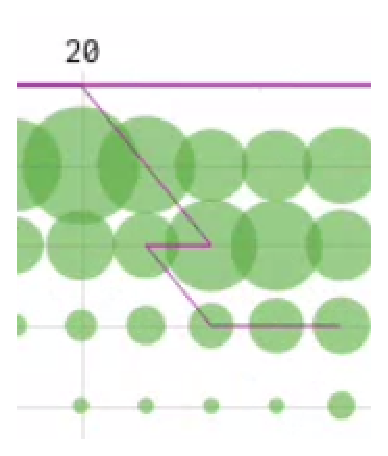
\includegraphics[width=2cm]{growing-family-weird}}

The lack of controls over the animation made it challenging to establish
how the vis. handled the cases were women gave birth to more than
one child at a given age, but by recording the vis. and scrubbing
through I found an example which is presented in the margin. The choice
to have the timeline double back is somewhat nonsensical, but it happens
rarely and does not impact the vis. significantly.

\pagebreak{}

\section{Visualization Design}

https://informationisbeautiful.net/visualizations/ransomware-attacks/

https://informationisbeautiful.net/visualizations/worlds-biggest-data-breaches-hacks/

The dataset I have chosen\footnote{\url{https://docs.google.com/spreadsheets/d/1wPgM8ye1AUTVxlZOFsyiKEPWp6iFt34xpp2XA5iM6P0/edit#gid=25233212}}
collects data relating to 361 separate ransomware attacks carried
out between 2013 and 2022. Most of the targets were commercial companies,
but some cities and other types of organisation are included. So we
are considering a table with each row representing an attack. Some
of the attributes in the table include:
\begin{itemize}
\item \textbf{Sector}. Categorical. The industry/field in which the organization
operates.
\item \textbf{Revenue}. Continuous. Revenue of the organization as of a
date specifide in a separate attribute.
\item \textbf{Ransom cost}. Continuous. Amount demanded by the ransomware.
\item \textbf{Ransom response.} Categorical; refused, paid, unkown.
\item \textbf{Year/month.} Ordinal.
\item \textbf{Location.} Categorical/geospatial. The country in which the
organization was based. This attribute has varying granularity, sometimes
just country, sometimes also the state/province.
\item \textbf{Ransomware}. Categorical; REvil, RansomEXX, unknown, etc.
The ransomware software or cyber criminal organization that perpetrated
the attack.
\item \textbf{Public/private company}. Categorical. Can be inferred from
the \textbf{stock symbol }attribute.
\item \textbf{Approx. number of employees}. Ordinal but specified as an
approximate range, e.g. 11-50, 10000+.
\end{itemize}
Some of the tasks a visualization of this data could support are as
follows:
\begin{itemize}
\item compare government/commercial organizations' typical responses to
ransomware
\item compare the openness of different types of organization
\item compare the strategies used by ransomware groups on different types
of organization, e.g. demanded ransom, size of organization targeted
\item explore trends in ransom attacks related to geopolitics
\item identify the most damaging attacks
\item compare the preferences for types of targets of different ransomware
software and groups
\item predict the characteristics that indicate a greater risk of ransomware
attack on an organisations
\item explore the trends in the size, cost, frequency of ransomware attacks
over time
\item identify clusters of successful ransomware attacks, i.e. contexts
in which ransomware attacks tend to be more successful
\end{itemize}
The above tasks are sufficiently distince and involve enough different
variables that I believe a dashboard of separate visualizations will
be most effective in supporting them all.

To support the task of exploring trends in ransomware over time I
would use a histogram with the month in the which the attack occurred
as the bin and the height of the bar indicating the number of attacks
that occurred in that month. I would also like to easily see what
proportion of those attacks were successful so I would use a group
of 3 bars for each month, one for attacks where the response was not
revealed, one for the number of attacks where the organization paid
out, and one for the number of ransoms that organisations refused
to pay.

To compare the different organization types and to include some insights
into the geopolitics of ransomware attacks I would create a separate
chart focused on the attributes 'sector', 'revenue', 'ransom response',
'approx number of employees', and possibly also 'location'. I would
infer a single numeric longitude for each attack based in on the 'location'
variable and encode this with horizonal position. I would encode the
revenue of the attacked company with vertical position. I would encode
the 'ransom response' with hue, green for refused, gray for unknown,
pink/red for ransom paid. The marker for each attack will be a line
and the orientation of the line will indicate the sector, $45^{\circ}$
for governmental $-45^{\circ}$ for commercial, such that clusters
of different types will create a distinct texture.
\end{document}
